\documentclass[UTF8,a4paper,11pt,fontset=none]{ctexart}
\usepackage[margin=2.1cm]{geometry}
\usepackage{fontspec,booktabs,tabularx,longtable,amsmath,amssymb}
\usepackage{graphicx,float,fancyhdr,xurl,fvextra,caption,placeins}
\usepackage[hidelinks]{hyperref}
\setmainfont{DejaVu Serif}
\setsansfont{DejaVu Sans}
\setmonofont{DejaVu Sans Mono}[Scale=0.86]
\IfFontExistsTF{Noto Serif CJK SC}{\setCJKmainfont{Noto Serif CJK SC}}{\setCJKmainfont{SimSun}[AutoFakeBold=2.5]}
\IfFontExistsTF{Noto Sans CJK SC}{\setCJKsansfont{Noto Sans CJK SC}}{\setCJKsansfont{Microsoft YaHei}}
\setCJKmonofont{Microsoft YaHei}
\ctexset{section={format=\Large\bfseries},subsection={format=\large\bfseries}}
\setcounter{tocdepth}{2}
\setlength{\parskip}{0.15em}
\linespread{1.02}
\setlength{\emergencystretch}{2em}
\renewcommand{\arraystretch}{1.22}
\raggedbottom
\pagestyle{fancy}
\fancyhf{}
\fancyhead[L]{\small 互联网数据库开发 · 个人作业 3}
\fancyhead[R]{\small 2413581 黄奕浩}
\fancyfoot[C]{\thepage}
\setlength{\headheight}{14pt}
\captionsetup{font=small,labelsep=quad}
\fvset{fontsize=\footnotesize,numbers=left,numbersep=7pt,frame=none,breaklines=true,breakanywhere=true,breakautoindent=true,tabsize=2}
\newcommand{\code}[1]{\texttt{#1}}
\hypersetup{pdftitle={WordPress校园学习网站布局与插件设计},pdfauthor={黄奕浩 2413581}}
\begin{document}
\begin{titlepage}
\thispagestyle{empty}\centering
\vspace*{.6cm}

\includegraphics[width=.43\textwidth]{figures/nankai_logo_color.png}
\vspace{.9cm}
\rule{.88\textwidth}{.8pt}\par\vspace{.55cm}
{\fontsize{28pt}{35pt}\selectfont\bfseries 互联网数据库开发课程实验报告\par}
\vspace{.65cm}
{\fontsize{21pt}{29pt}\selectfont\bfseries 个人作业 3\quad 开源建站工具初试\par}
\vspace{.55cm}\rule{.88\textwidth}{.8pt}\par
\vspace{1.55cm}
{\fontsize{19pt}{28pt}\selectfont\bfseries 姓名：黄奕浩\qquad 学号：2413581\par}
\end{titlepage}
{\small\tableofcontents}
\clearpage

\section{站点内容组织与页面设计}
\subsection{网站定位与栏目安排}
知行学习小组网站围绕校园学习与团队展示组织内容。首页用于说明团队定位，并展示最近发布的学习记录；团队介绍页面说明成员与工作内容；学习资源页面归纳课程知识；学习计划页面提供可操作的任务清单。四个入口分别承担介绍、浏览、查阅和记录进度的作用，页面之间通过顶部导航联系起来。

内容采用文章与固定页面两种形式。三篇文章分别为“SQL 查询练习记录”“前端交互实践记录”和“团队协作与学习计划”，用于记录具体的学习过程。团队介绍、学习资源和学习计划作为固定页面，保留在导航中。这样既能持续补充文章，又能让主要栏目保持稳定。

\subsection{首页布局与阅读顺序}
首页自上而下分为导航、首屏介绍、最新学习记录和页脚。导航左侧显示“知行 / 学习小组”，右侧提供团队介绍、学习资源和学习计划三个入口。首屏展示团队主题及简短说明，按钮直接进入学习资源页面。首屏之后排列三篇文章，让访客先了解网站用途，再选择需要阅读的内容。

文章列表使用三列网格，每张卡片包含发布日期、文章标题和摘要。标题链接进入对应文章，摘要由 WordPress 的文章循环读取。页面主体的最大宽度为1120像素，并通过居中与左右留白控制阅读范围。页脚显示团队名称、姓名和学号，与顶部品牌信息相呼应。

\begin{figure}[H]\centering
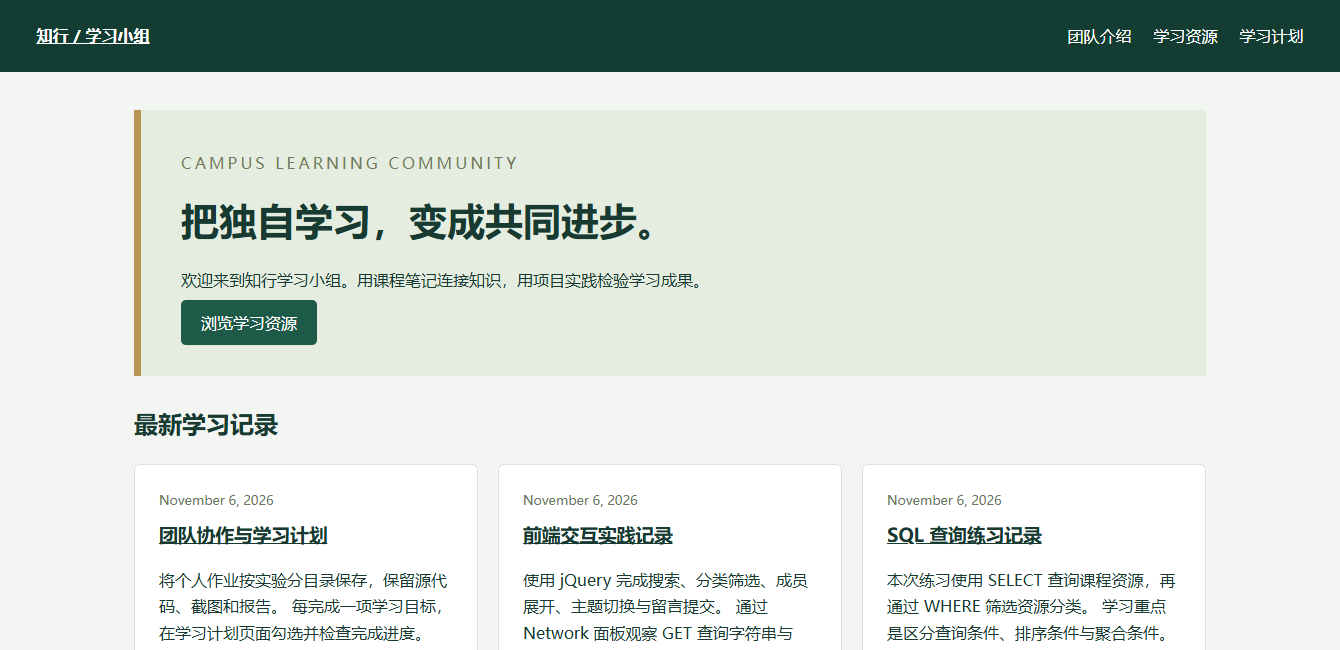
\includegraphics[width=\linewidth,height=.48\textheight,keepaspectratio]{figures/figure-03.png}
\caption{校园学习网站首页与三篇学习记录}
\end{figure}


\subsection{团队介绍与学习资源页面}
团队介绍采用团队说明与成员信息两级结构，展示黄奕浩及学号2413581，并说明前端交互、原型设计、插件开发和建站记录等工作。页面以文字为主，便于直接查阅成员信息。

学习资源按数据库、Web前端和协作工具三个主题组织。数据库部分列出 SELECT、JOIN、GROUP BY 与索引；前端部分围绕 HTML、CSS、jQuery 和 AJAX；协作工具部分介绍 Git 和浏览器开发者工具。各主题使用二级标题分隔，使访客可以按知识方向定位内容。

\begin{figure}[H]\centering

\includegraphics[width=\linewidth,height=.36\textheight,keepaspectratio]{figures/figure-04.png}
\caption{团队介绍页面}
\end{figure}


\begin{figure}[H]\centering
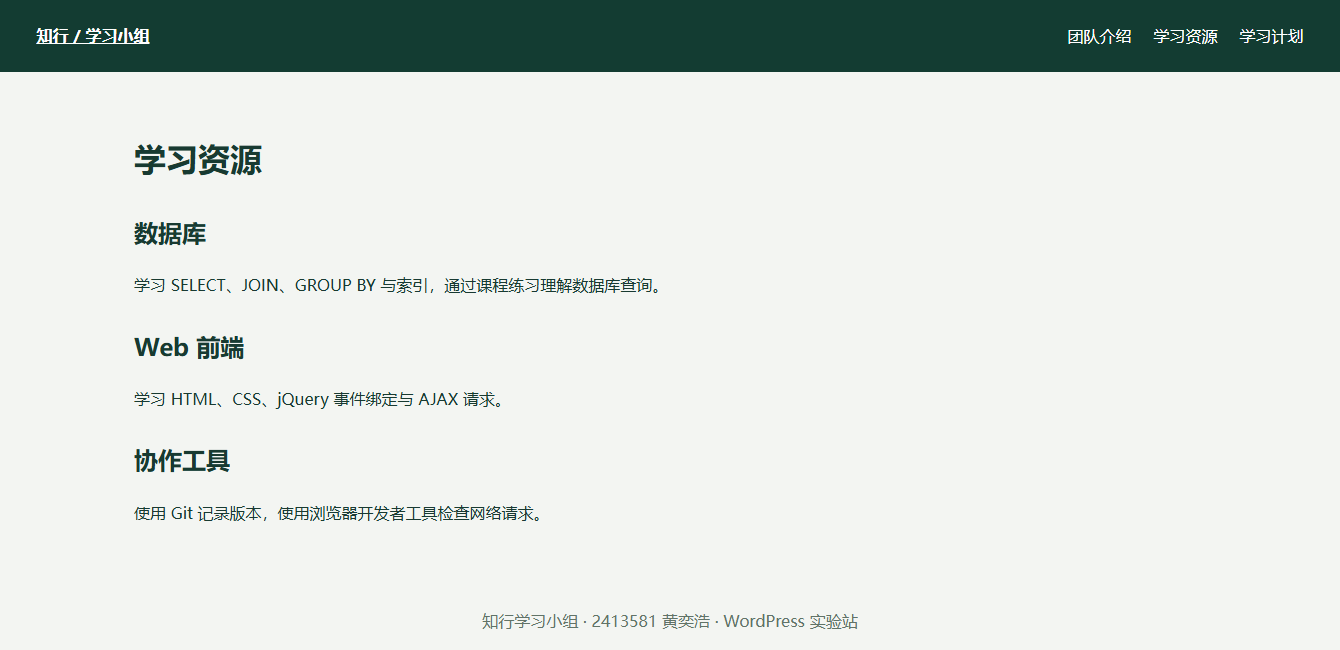
\includegraphics[width=\linewidth,height=.36\textheight,keepaspectratio]{figures/figure-05.png}
\caption{学习资源页面}
\end{figure}


\section{主题结构与动态页面生成}
\subsection{主题文件的职责}
自制主题“知行校园学习空间”由样式、主题功能和页面模板组成。style.css 保存主题名称、作者和版本等识别信息，同时定义导航、首屏、文章卡片及正文区域的样式。functions.php 注册样式加载逻辑和主题支持，index.php 负责根据当前请求输出首页、文章或固定页面。

functions.php 在 wp\_enqueue\_scripts 钩子中调用 wp\_enqueue\_style，将主题样式交给 WordPress 统一加载；get\_stylesheet\_uri 返回当前主题的样式地址。主题声明 title-tag 和 post-thumbnails 支持，并注册名为 primary 的导航位置。当前页面模板直接输出三个主要栏目的链接。

\subsection{首页与正文页面的生成流程}
页面模板先输出文档头、导航和主体容器，再通过 is\_front\_page 判断当前是否为首页。首页显示首屏介绍，并在 have\_posts 与 the\_post 构成的文章循环中逐条输出文章卡片。卡片通过 get\_the\_date、the\_title、the\_excerpt 和 the\_permalink 取得日期、标题、摘要及详情链接。

访问文章或固定页面时，模板进入另一条分支，在正文区域输出标题和 the\_content 的内容。学习计划页面中的短代码也在正文处理过程中执行，因此同一套页面模板既能显示普通文字，也能显示插件生成的交互模块。修改后台内容后，前台读取的仍是 WordPress 保存的文章或页面数据。

\subsection{栏目链接与输出处理}
团队介绍、学习资源和学习计划的页面编号分别保存在 zx\_team\_page、zx\_resource\_page 和 zx\_plan\_page 选项中。模板通过 get\_option 读取编号，再由 home\_url 生成带 page\_id 参数的地址。导航入口因此由站点中的页面记录决定。

模板对生成的链接使用 esc\_url，对日期文字使用 esc\_html。学习计划插件中的任务编号使用 esc\_attr，任务文字使用 esc\_html。链接、HTML属性和可见文字分别采用对应的输出处理方式。

\subsection{视觉样式与窄屏布局}
网站以深绿色区分导航和主要按钮，浅绿色首屏承载团队介绍，白色卡片呈现学习记录。正文使用微软雅黑及系统后备字体，行高设为1.65。标题、正文和日期采用不同字号与间距，使内容层次在同一页面内保持清楚。

样式表使用760像素作为窄屏断点。当页面宽度低于这一值时，文章网格由三列变为单列，首屏标题由38像素调整为28像素，页头改为纵向排列。上述变化由 CSS 媒体查询完成，使卡片和导航适应较窄的显示区域。

\section{学习计划插件设计与实现}
\subsection{模块启用与短代码入口}
网站启用了 SQLite Database Integration 和自制“知行学习计划”插件。前者提供数据库适配，后者将任务清单作为独立业务模块提供给页面。主题负责整体显示，业务插件负责学习计划，两者通过 WordPress 的正文与短代码机制连接。

\begin{figure}[H]\centering
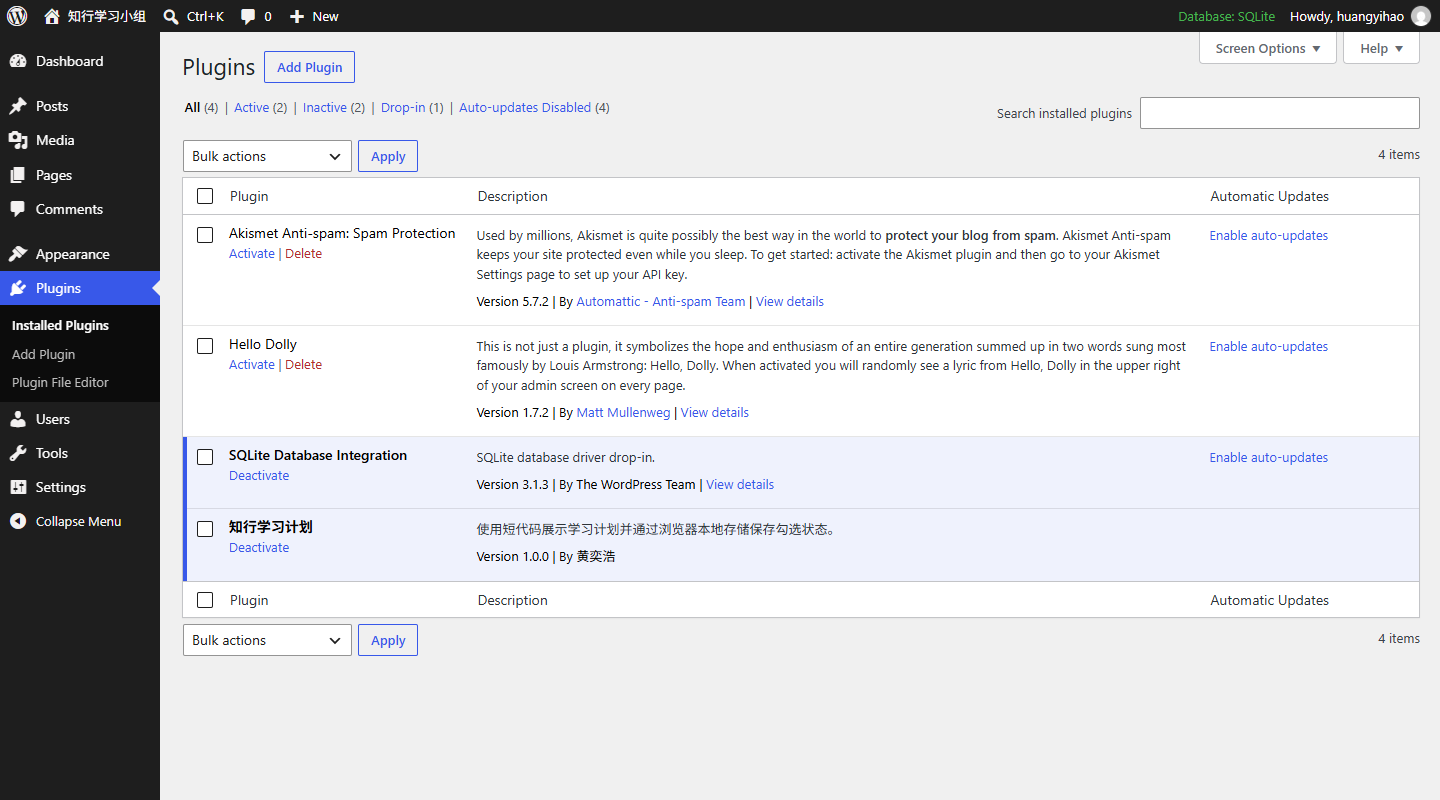
\includegraphics[width=\linewidth,height=.36\textheight,keepaspectratio]{figures/figure-06.png}
\caption{后台已启用的插件}
\end{figure}


\begin{figure}[H]\centering
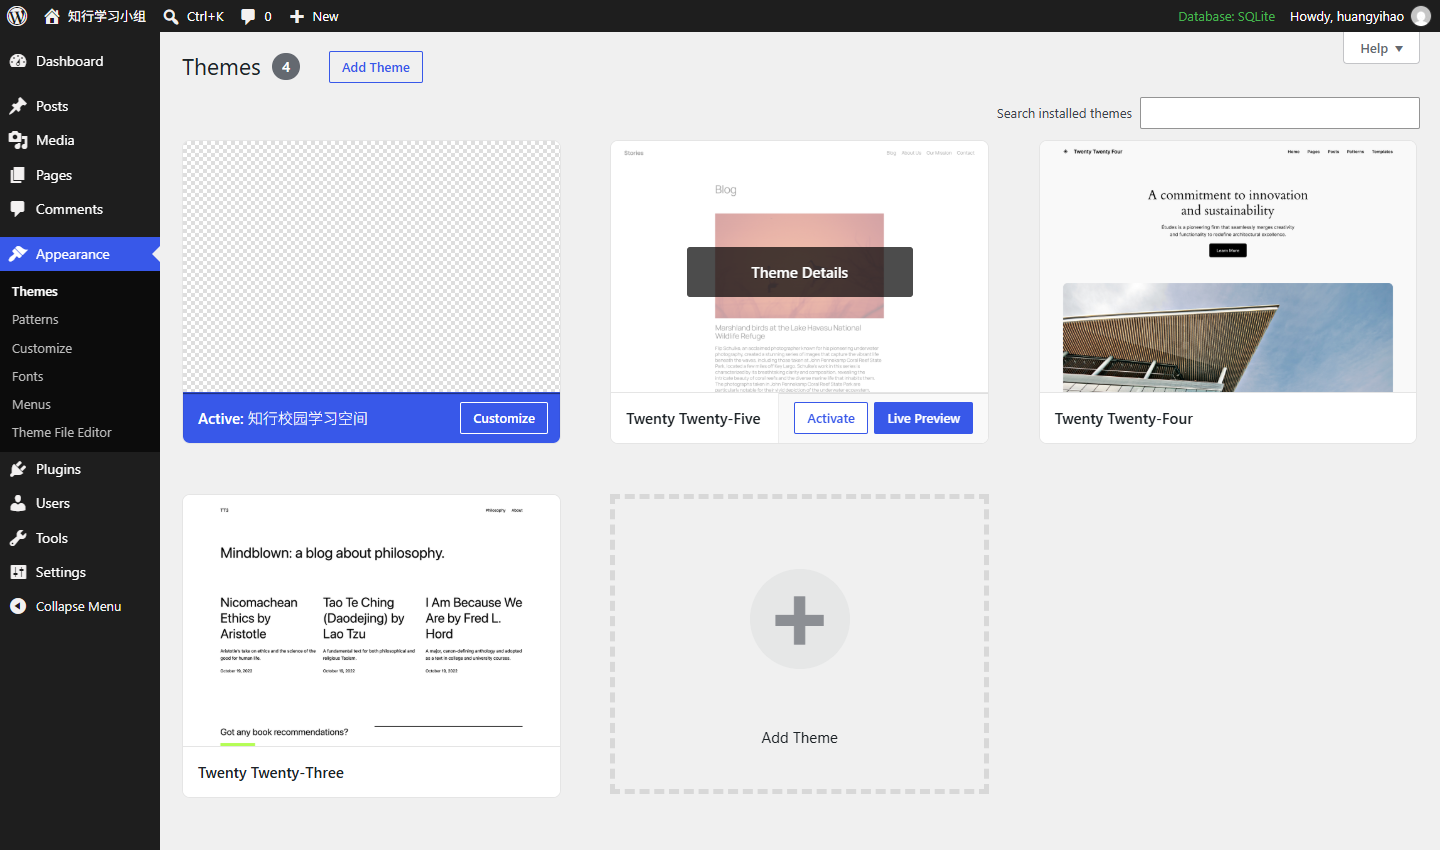
\includegraphics[width=\linewidth,height=.36\textheight,keepaspectratio]{figures/figure-07.png}
\caption{后台已启用的知行主题}
\end{figure}


学习计划插件使用 add\_shortcode 绑定短代码与页面生成函数。页面正文中的调用形式为：
\begin{center}\code{[zhixing\_plan]}\end{center}
WordPress 处理正文时调用对应函数。函数使用输出缓冲生成 HTML，再通过 ob\_get\_clean 返回结果。页面编辑内容只需保留短代码，任务界面的生成逻辑集中在插件中。

\subsection{任务清单与完成进度}
插件定义四项任务：完成GET与POST请求分析、完成五项jQuery交互练习、整理页面设计与模板选择，以及完成WordPress建站记录。PHP 循环为每项任务生成一个复选框，并用 data-task 属性保存任务编号。界面在任务列表下方显示“已完成 C / 4 项”。

设第 $i$ 项任务的勾选状态为 $x_i$，已勾选时取1，否则取0，则完成数为
\[
C=\sum_{i=1}^{4}x_i.
\]
脚本读取当前所有复选框，以 checked 属性筛选已勾选项，并将筛选结果的数量写入进度文本。每次触发 change 事件后重新计算，因此勾选和取消勾选都会立即反映到显示结果中。

\begin{figure}[H]\centering
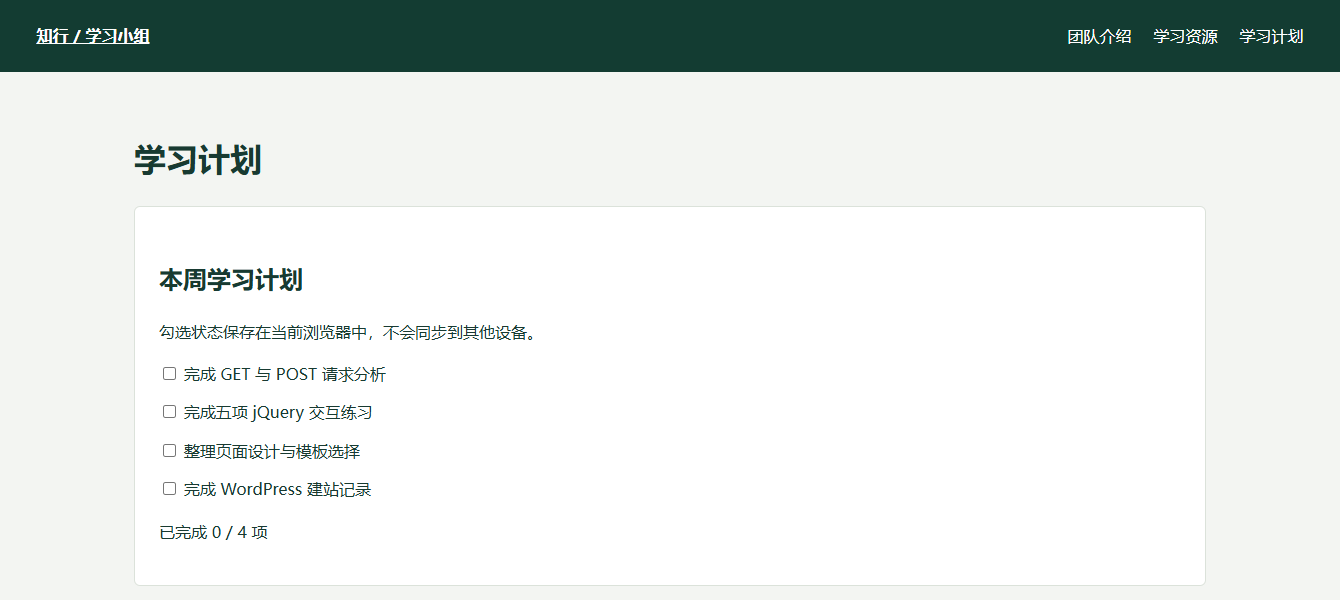
\includegraphics[width=\linewidth,height=.36\textheight,keepaspectratio]{figures/figure-08.png}
\caption{学习计划的初始状态}
\end{figure}


\begin{figure}[H]\centering
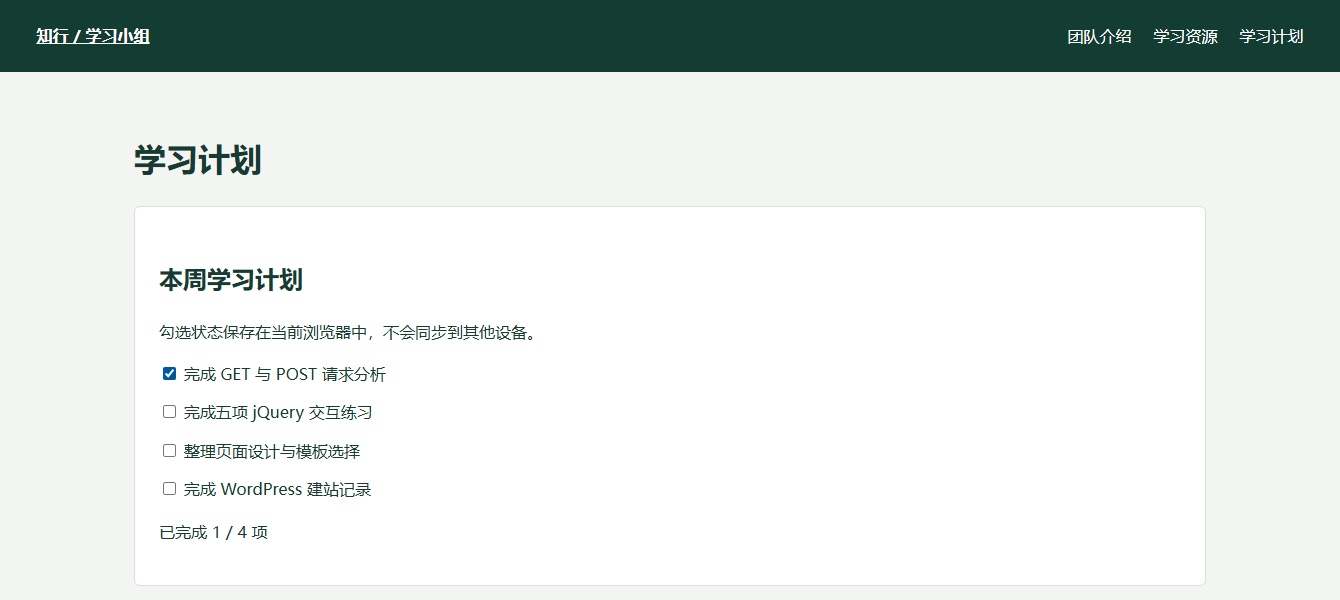
\includegraphics[width=\linewidth,height=.36\textheight,keepaspectratio]{figures/figure-09.png}
\caption{勾选一项任务后显示已完成1/4项}
\end{figure}


\subsection{勾选状态的保存与恢复}
学习进度以 zx-plan 为键保存在当前浏览器的 localStorage 中。保存内容是任务编号到布尔值的对应关系，JSON.stringify 将其转换为字符串；页面重新打开时，通过 JSON.parse 恢复对象，并逐个设置复选框的 checked 属性。

初始化时，脚本先读取已保存的状态，再绑定 change 事件，最后更新一次进度。触发事件后，脚本同时更新状态对象、写入本地存储并刷新进度文字。读取和写入均使用 try/catch 包围，读取失败时保留空状态作为初始值。学习计划的勾选状态按浏览器分别保存。

\section{后台内容维护与前台呈现}
\subsection{文章与固定页面的维护}
学习记录以文章发布，团队介绍、学习资源和学习计划以固定页面维护。后台修改文章标题或正文后，首页的文章卡片与详情页读取更新后的内容。固定页面的正文可分别调整团队说明、资源分类和计划模块所在位置。

学习计划页面保存短代码，插件文件保存任务清单和交互逻辑。需要修改页面介绍文字时编辑页面正文，需要调整任务内容时修改插件中的任务数组。这样将页面内容与模块实现分别组织，便于对应具体修改的位置。

\begin{figure}[H]\centering
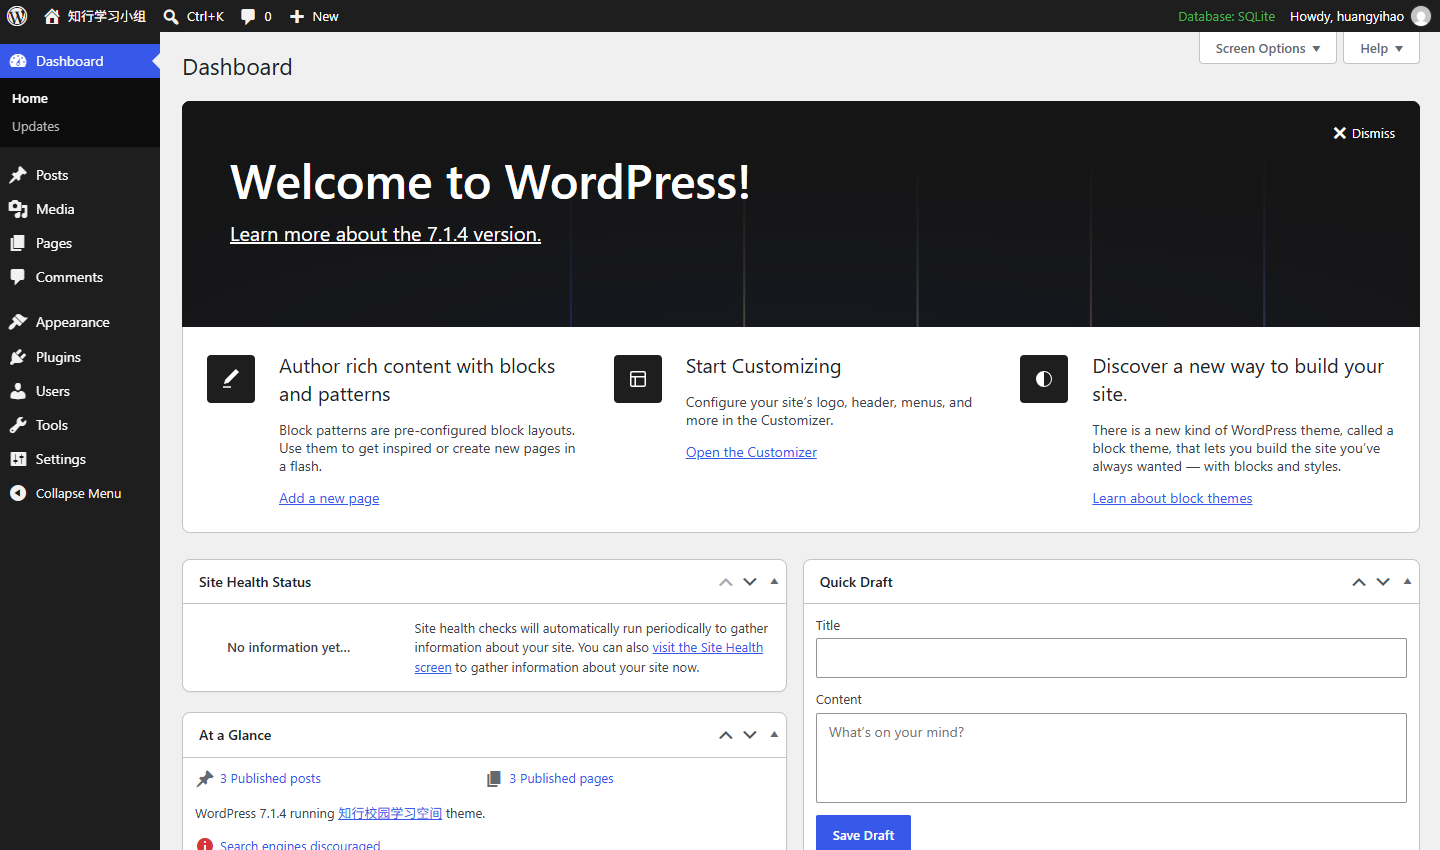
\includegraphics[width=\linewidth,height=.36\textheight,keepaspectratio]{figures/figure-10.png}
\caption{WordPress后台的文章与页面管理入口}
\end{figure}


\subsection{页面运行效果}
首页显示三篇学习记录，顶部导航能够进入团队介绍、学习资源和学习计划。文章卡片提供标题和摘要，固定页面显示对应栏目正文。计划模块从未勾选的0/4项变为勾选后的1/4项，刷新页面后继续显示已保存的选择。

页面布局、动态内容和业务插件共同构成最终站点：主题统一导航、首屏与正文区域；文章和页面提供学习内容；插件将静态计划文字扩展为可操作的任务清单。各部分在同一导航结构下呈现，形成校园学习与团队展示网站。

\FloatBarrier\clearpage\appendix
\section{核心源程序}
\subsection{主题功能注册}
\VerbatimInput{code/theme-functions.php}
\subsection{学习计划插件}
\VerbatimInput{code/source-01.php}
\end{document}
